\documentclass[a4paper,11pt]{article}

\usepackage{amssymb}
\usepackage{amstext}
\usepackage{amsmath}
\usepackage{amsthm}
\usepackage{booktabs}
\usepackage{graphicx}
\usepackage{float}
\usepackage{url}

\usepackage{xcolor}
\newcommand{\bluenote}[1]{\color{blue}{ \em #1 }\color{black}}

\usepackage{geometry}
 \geometry{
 a4paper, %letterpaper,
 total={17cm,22.8cm},
 margin=24mm,
 top=22.4mm,
 bottom=25.4mm
 }
 
% Times new roman
\usepackage{mathptmx}

\usepackage[T1]{fontenc}

\thispagestyle{empty} 

\setlength{\parindent}{0pt}


\author{%
%  \fontsize{10}{12}\selectfont
  \begin{minipage}[t]{0.47\textwidth}
    \centering
    Samar Rahmouni \\ srahmoun@andrew.cmu.edu
  \end{minipage}
  \and
  %
  \begin{minipage}[t]{0.45\textwidth}
    \centering
    Advisor: Prof. Giselle Reis \\ giselle@cmu.edu
  \end{minipage}%
  \vspace*{2ex}
}


\date{}

\title{{\Large\sc Senior Thesis 2021-22\\[2ex]}{\LARGE\bf Prospectus\vspace*{3ex}}}


\begin{document}

\maketitle 

\section{Problem and Overview of the Proposed Solution}
Reinforcement learning, though a powerful and simple trial-and-error procedure that found a lot of success in games like Go, cannot be deployed in the real world 
because of the lack of security guarantees. For instance, though an autonomous car trained with reinforcement learning is bound to learn how to drive, the AI needs to crash 
to learn that crashing is not desirable. 

\medskip

In the context of the proposed thesis, we investigate both the security and the interpretability aspect of reinforcement learning in a cooperative adaptive cruise control inspired from \cite{vnc20},
in the aim of finding how formal security frameworks can guide the representation, robustness and extrapolation of knowledge in Reinforcement
Learning agents. We do so by experimenting and comparing both the optimization and security of three different RL implementations. 

\medskip

The first is a basic tabular Q-learning where we expect no security guarantees. The second is a hybrid architecture that incorporates the safe controller in \cite{vnc20} in a RL architecture. 
The safe controller (SC) returns a range of safe velocities given the current state of the environment. The SC then constricts the possible actions of the RL continuously at every given time step and the role of the RL is purely 
to find the optimal velocity in the safe range to minimize the distance between the cars in the platooning scenario. The third is what we will define as a logic-based inference RL. We investigate learning inferences rules in a deterministic environment 
where the result of an action given a state is not dependent on any probabilistic event. We approach the problem using inductive reasoning where the goal is to incorporate the learned rule knowledge into the decision making of a tabular Q-learning RL agent. 
In the given scenario, this will make use of the SC to develop a mapping from the state representation to a reward scheme, i.e. punish before a crash is bound to happen and adapt the Q-value and the epsilon-greedy approach. 

\section{Significance}
Implementing a robust adaptive controller that is effective in terms of precision, time, and quality of decision
when facing dynamic and uncertain scenarios, has always been a central challenge in AI and robotics.
As autonomous cars are deployed, IoT is popularized, and human-robot interactions become more complex, we
are more and more confronted with the need for robotic agents that can effectively and continually adapt
to their surroundings, not only in simulation, but also in practice, when deployed as a cyber-physical system. 
Since we are unable to provide a repertoire of all possible scenarios and actions,
our agents need to be able to autonomously predict and adapt to new changes. RL is an approach that
supports developing these capabilities, it is also the solution that AlphaGo, Deepmind AlphaStar, and OpenAI Five have
adopted \cite{li2019reinforcement} and found success in. 
However, as RL is a trial-and-error process, a car trained using RL is bound to crash to learn not to crash again. Safe Reinforcement Learning is then crucial 
to investigate in order to be able to deploy it in larger scales, but also out of simulation. 
\cite{kurdkelly2003} lays the foundations of verifications goals for Artificial Neural Networks (ANNs) to be ensured for safety-critical tasks. The need for this behavioral constraints stems from the inability to analyze and 
describe the behavior of NNs. The same argument translates to RL. In general, reinforcement learning does not any of the verification conditions in \cite{kurdkelly2003}. 
The observable behavior of a RL agent is unpredictable (e.g. AlphaGo gamestyle) and will more than not take hazardous actions since it is a trial-and-error process. Hence, it is important to investigate
the use of verified safety controller and the interpretability of RL in order to achieve these verifications goals.  


\section{Background and Related Work}
One of the many ways safety has been approached is by formalization and symbolic reasoning. 
In the case of artificial intelligence, recent work proposes Neurosymbolic integration. 
Neurosymbolic integration has been an ongoing work in the last years towards a combination of Deep Learning and Symbolic Reasoning.
The work has been a response to critics of DL, precisely, the lack of formal semantics and intuitive explanation and the lack of expert knowledge towards guiding machine learning models. 
Key questions the field targets are identifying the necessary and sufficient building blocks of AI \cite{garcez2020neurosymbolic}, namely, how can we provide the semantics of knowledge, 
and work towards meta-learning? Meta-learning in reinforcement learning is the problem of learning-to-learn, which is about efficiently
adapting a learned policy to conditions and tasks that were not encountered in the past. In RL, metalearning
involves adapting the learning parameters, balancing exploration and exploitation to direct the
agent interaction \cite{gupta_meta-reinforcement_2018,schweighofer_meta-learning_2003}. Meta-Learning is a central problem in AI, since an agent that can solve more
and more problems it has not seen before, approaches the ideal of a general-purpose AI. 

\medskip

Current Neurosymbolic AI trends are concerned with knowledge representation and reasoning, namely, they investigate computational-logic systems 
and representation to precede learning in order to provide some form of incremental update, e.g. a meta-network to group two sub-neural networks. \cite{Besold2017NeuralSymbolicLA}
This leads to neurosymbolic AI finding various applications including vision-based tasks such as semantic labeling \cite{vinyals2015, karpathy2015}, 
vision analogy-making \cite{Reed2015DeepVA}, or learning communication protocols \cite{Foerster2016LearningTC}.
However, such representation has not yet been investigated in tabular reinforcement learning algorithms. Precisely, the problem of knowledge extraction and interpretability of RL architecture is yet to be tackled.

\medskip

Artificial intelligence has moved away in the past years from symbolic to data-driven. 
Data-driven AI have proven both efficient and their algorithms easy to reuse. However, 
we are facing the limitations of such AI today whether 
in its incapability of developing abstract relations between components, or in the consistent problem of meta-learning in extrapolating learned knowledge 
in one environment to another, or finally, the safety properties that are harder to reason about and furthermore ensure. 
In the light of such limitations, hybrid architectures are becoming increasingly popular \cite{garcez2020neurosymbolic}. 

\medskip

However, most approaches so far only considered neural networks. In \cite{urban2021}, they present multiple formal methods that have been investigated 
and applied to Machine Learning, these include SMT-based and MILP-based formal methods which use constraint satisfaction and mixed-integer linear problems. The main idea is to reduce safety properties into a set of 
constraints. If a solution exists then the property does not hold, else it is safe. 
These methods, though sound and complete, do not scale for bigger networks.

\medskip

Approaches that were concerned with safe reinforcement learning rather than the above, have approached the problem in previous work \cite{Garca2015ACS} in two ways. 

First was changing the optimization criteria \cite{rockafellar2000}, precisely by incorporating risk into the performance of the policy.
Namely, either considering the worst case scenario and constraining on it, reducing the variance to be more sensitive or applying constraints i.e. only update the policy if the action is in a safe set. 
This does not however guarantee safety, but tends to minimize the probability of risk, hence not allowing RL systems to be deployed in the physical world. 
Second was to consider the exploration process, either by incorporating external knowledge i.e. learning from demonstration \cite{Siebel2007EvolutionaryRL} or adopting a risk directed exploration \cite{law2005}. These approaches can be considered rigid, 
as requiring more data and expert knowledge that needs to be proven safe and sound, or in the latter, decreasing the efficiency and requiring more time for the learning process. 
In particular, in these previous two approaches, work that makes use of formal security frameworks is yet to be investigated. 

\medskip

Some of the more recent work that does investigate a hybrid architecture (i.e. RL and symbolic reasoning) makes use of
set-theoretic techniques and constraint satisfaction problems to optimize from the constraints \cite{Li2021SafeRL}, or proposes a reactive system called a shield \cite{alshiekh2017} to either constraint the actions given by the environment or adapt them once the RL module chooses one. 
In both cases, the added safety controller is described by its specifications, rather than being an independent existing controller. 
\newline 
Our approach is novel as it (1) focuses on tabular reinforcement learning rather than neural networks, (2) provides a framework independent of the specifications of either 
the reinforcement learning controller or the safe controller and (3) investigates a translation from  
symbolic compositional state representation in RL to logic-based inference. 

\section{Research Contribution}
We (1) provide a framework to incorporate a verified safety controller into a Reinforcement Learning architecture, 
(2) investigate a compositional state representation for Reinforcement Learning in the lines of classical planning, 
and (3) incorporate rule knowledge into the decision-making of tabular Reinforcement Learning in a deterministic environment. 
The above is done as to test and experiment on the tradeoff of optimization and safety in basic RL, RL with a safe controller, 
and finally a logic-based inference RL.


\section{Evaluation Plan and Timeline}
The project will proceed in two phases. The first focuses on the implementation of the reinforcement learning controller along with 
connecting the safe controller. Precisely, we proceed with the following. 
\begin{enumerate}
  \item Formalizing the car platooning scenario as an optimization problem for the RL agent. [7th October] 
  \item Concretizing the architecture and describe the relations between components. [8th October]
  \item Implementation of the RL controller independently of the safe controller. [20th October]
  \item Modeling the states as a propositional formula in the lines of classical planning in order to match the safe controller specifications. [26th October]
  \item Implementation of the framework to map from Maude to Python, after feeding the state representation into the safe controller. [10th November]
  \item Experimenting and testing the optimization results of the RL controller with and without the safety guarantees of the safe controller. [20th November]
\end{enumerate}

The second phase focuses on the possible inferences of safety properties in a deterministic environment given a compositional propositional formulas
state representation. 
\begin{enumerate}
  \item Investigate learning inference rules [state given action] in a deterministic environment. [5th February]
  \item Incorporate rule knowledge into decision making of a tabular RL precisely by looking into a hybrid architecture that makes use of 
        symbolic AI to adapt the Q-values table and/or the epsilon-greedy algorithm. [7th March]
  \item Develop a mapping from compositional state representation to reward schemes given safe controller outputs. [10th April]
  \item Experimenting and testing the optimization and safety results of the RL controller with modified rewards. [20th April]
\end{enumerate}

Given these two phases, we want to compare both approaches (i.e. RL with safe controller and logic-based inference RL) into balancing between safety guarantees and optimization. 
Both phases will use the car platooning as a main scenario for implementation and testing. Below is a gannt chart of the expected timeline. \newline 


\begin{figure}[H]
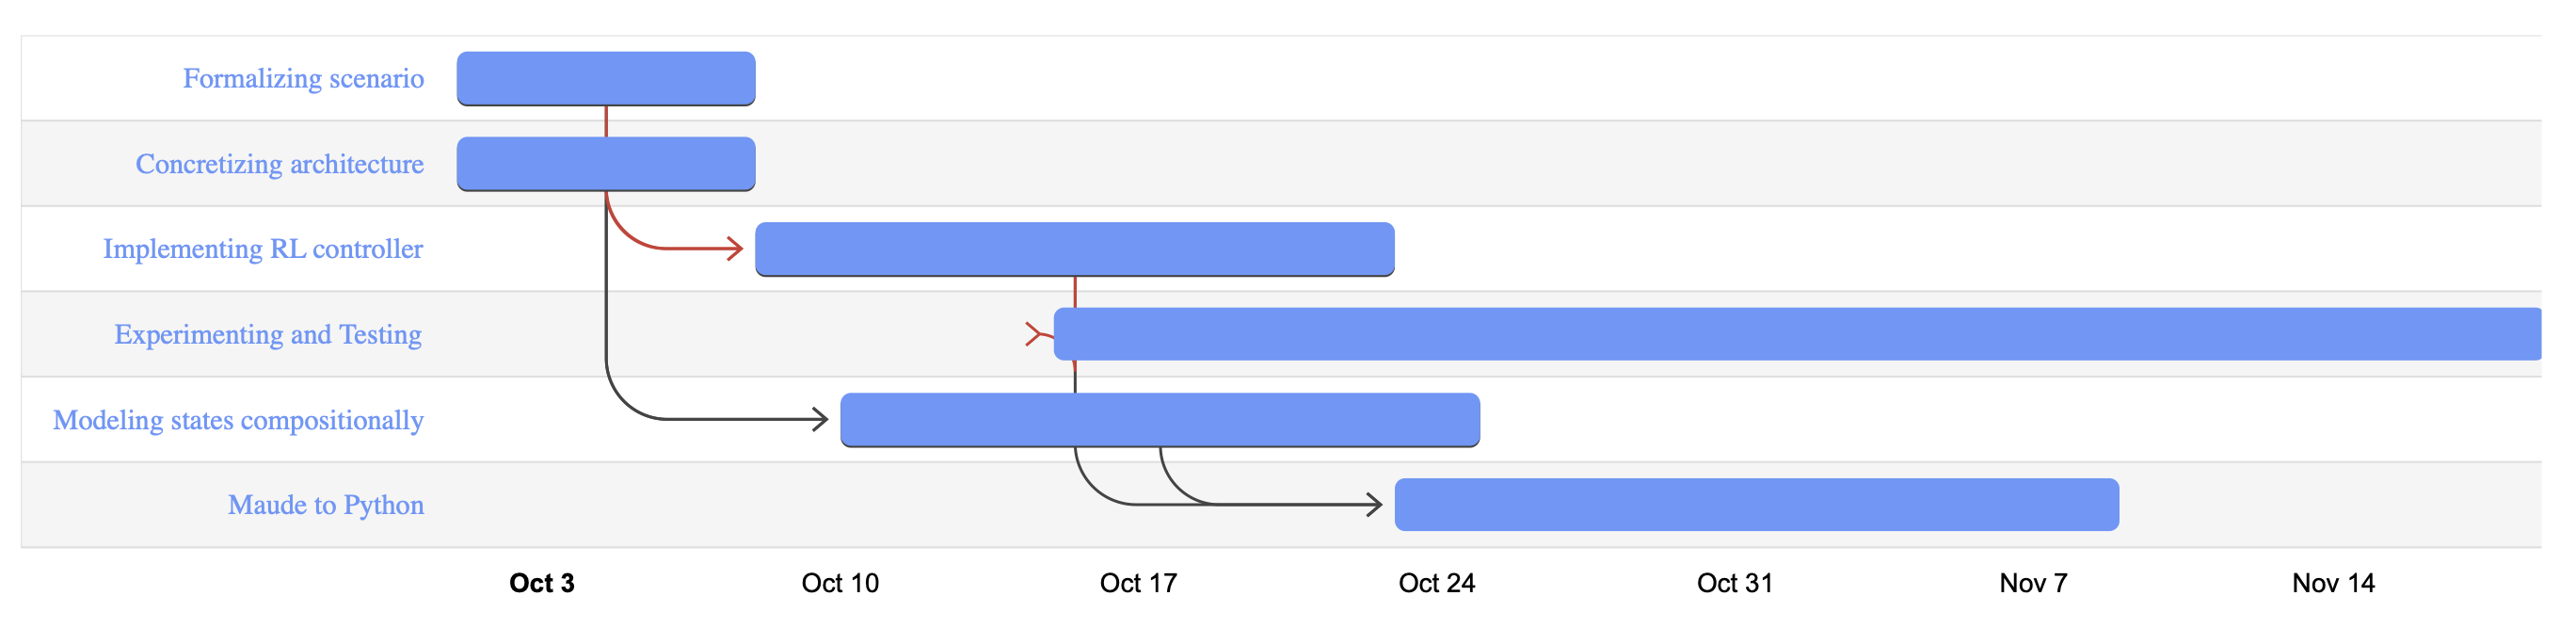
\includegraphics[scale=0.18]{phase-1.png}  
\caption{Timeline for Phase 1}
\label{fig:phase-1}
\end{figure}

\begin{figure}[H]
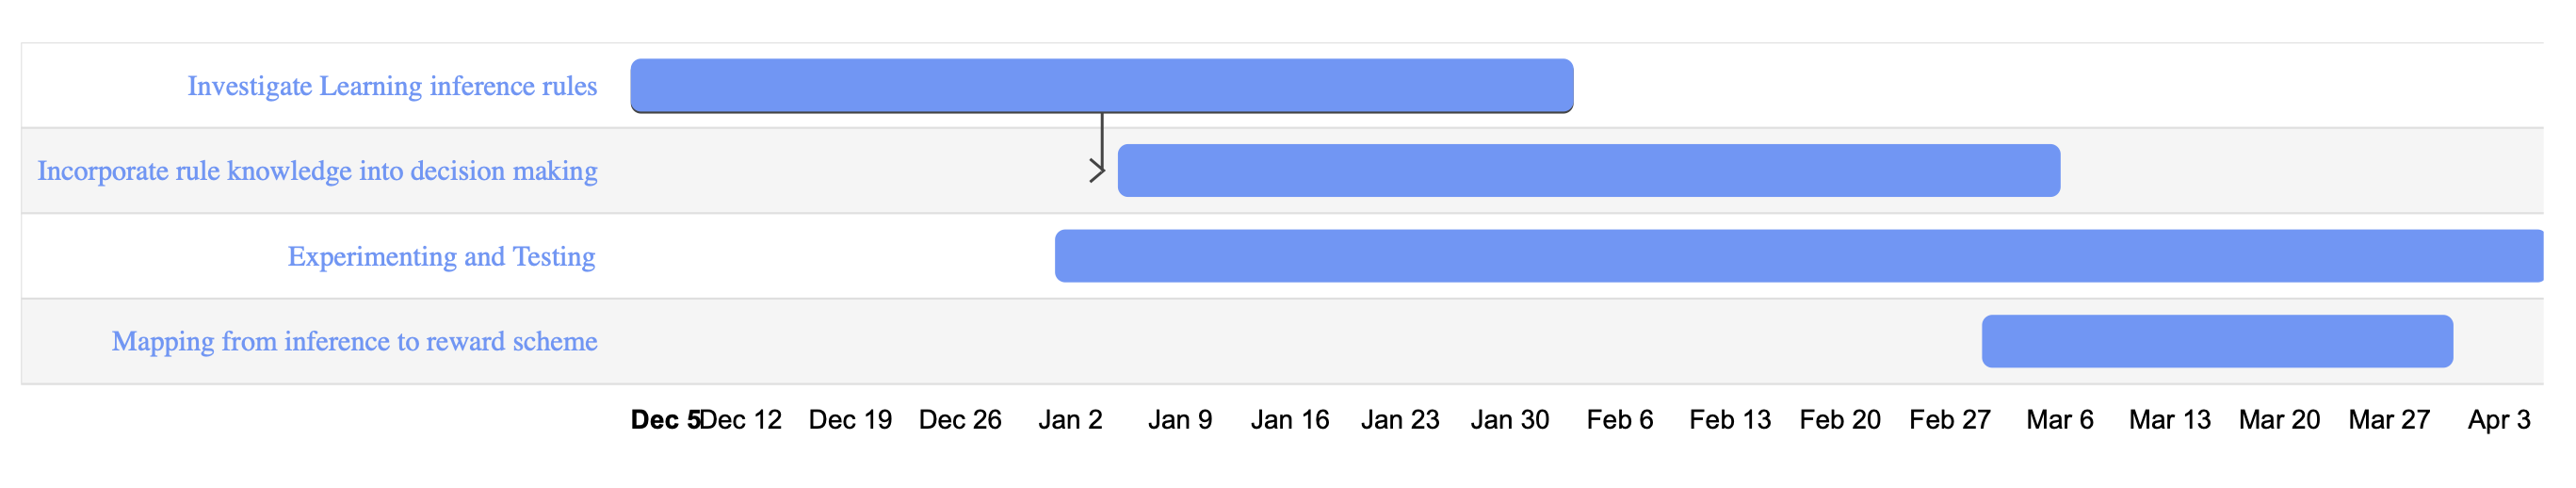
\includegraphics[scale=0.18]{phase-2.png}
\caption{Timeline for Phase 2}
\label{fig:phase-2}
\end{figure}

\newpage

\bibliographystyle{unsrt}
\bibliography{biblio.bib}



\end{document}
